\section{Installation and first steps}
\label{tutorial_02}

\subsection{Installation}

Start off by installing BMotion Studio. BMotion Studio is a fix part of the ProB Installation and is available as a plugin for the Rigorous Open Development Environment for Complex Systems (RODIN).

\subsubsection{Step 1: Install Rodin for the first time}

\tick{You can skip this step and go on with step 2 if you have already downloaded Rodin.}

The first step is to download Rodin. Rodin is available for download at the Rodin Download page (\ref{rodin_download})

Rodin is available for Windows, Mac OS, and Linux.  No matter which platform you use, the distribution is always packed in a zip-file (\ref{zip_file}).  Download the zip file for your system anywhere on your PC.

\info{It is recommended that you download the latest stable version.}

For a detailed documentation about Rodin we refer to the official Rodin hanbdook page \href{http://handbook.event-b.org}{http://handbook.event-b.org}.

\subsubsection{Step 2: Install BMotion Studio for the first time}

Step: Start Rodin and select \textsf{Open Help $\rangle$ Install New Software...} (compare with figure \ref{fig_tut_02_install1}). Select the ProB Update site (http://www.stups.uni-duesseldorf.de/prob\_updates) and install ProB for Rodin2 Click on the \textsf{$Next >$} button and follow the installation instruction.

\begin{figure}[!h]
\begin{center}
	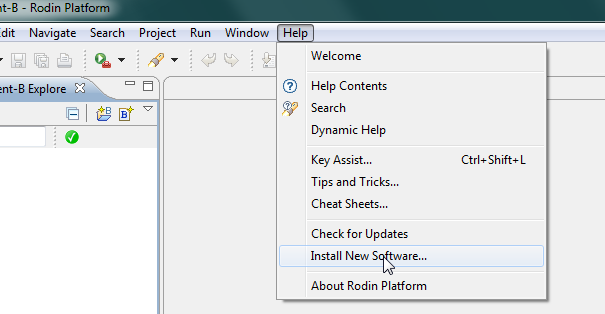
\includegraphics{img/tutorial/tut_02_install1.png}
	\caption{Install New Software for Eclipse or Rodin respectively}
	\label{fig_tut_02_install1}
\end{center}
\end{figure}

\subsection{The First Visualization: A Waterboiler Model}

\tick{\textbf{Goals:} The objective of this section is to learn how to create a visualization for a Event-B of a waterboiler model. The waterboiler has functions to open/close its cap, to fill/effuse water and to switch on/off.}

\subsubsection{Waterboiler Model}

Since BMotion Studio allows to create a visualization for existing Event-B models, we have to import the initial Event-B model of the waterboiler: 

\begin{enumerate}
	\item Step: Download the \file{Waterboiler.zip}{Waterboiler.zip}.
	\item Step: Select \textsf{File $\rangle$ Import}. A window should popup as shown in figure \ref{fig_tut_03_waterboiler1}.
	\item Step: Select \textsf{General $\rangle$ Existing Project into Workspace} and click on the \textsf{$Next >$} button.
	\item Step: Mark \textsf{Select archive file}, select the \texttt{Waterboiler.zip} file and click on the \textsf{Finish} button. 
\end{enumerate}

\begin{figure}[!h]
\begin{center}
	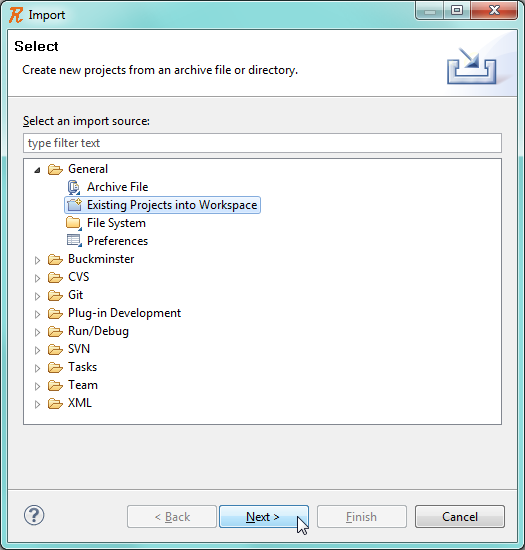
\includegraphics{img/tutorial/tut_03_waterboiler1.png}
	\caption{The Eclipse import wizard}
	\label{fig_tut_03_waterboiler1}
\end{center}
\end{figure}

You should see the Waterboiler project in your workspace now.

\subsubsection{Creating a new BMotion Studio Visualization}

Open the context menu of the Lift Event B project and select \textsf{New $\rangle$ Other}. This should bring the project wizard of Eclipse where you can create other files/projects beside a new BMotion Studio Visualization. Select \textsf{BMotion Studio $\rangle$ BMotion Visualization} and click on the \textsf{$Next >$} button. as shown in figure \ref{fig_tut_03_waterboiler2}. 

\begin{figure}[!h]
\begin{center}
	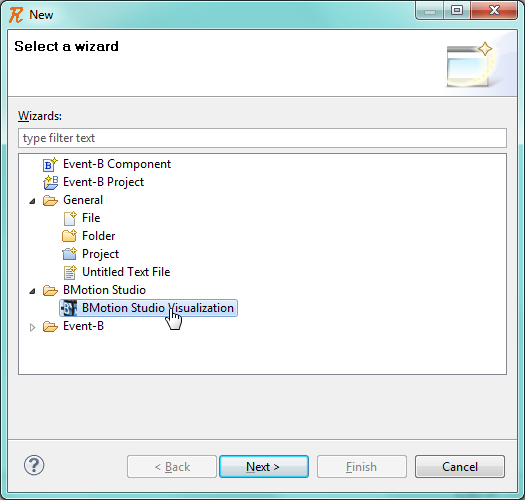
\includegraphics{img/tutorial/tut_03_waterboiler2.png}
	\caption{Creating a new BMotion Studio Visualization}
	\label{fig_tut_03_waterboiler2}
\end{center}
\end{figure}

This should bring up the \textsf{New BMotion Studio Visualization wizard} where you have to enter the relevant data needed for creating a new visualization as shown in figure \ref{fig_tut_03_waterboiler3}. The first required field is the Project name field which allows to select a project. Since, we opended the New BMotion Studio Visualization wizard via an exisisting Event B project, the corresponding project should be preselected. In the next field (BMotion Studio Visualization filename) you have the option to enter a valid, i.e. non empty and non-existing name for your visualization, i.e. "VWaterboiler". In a final step you have to select the machine for which you want to create a visualization in the table at the bottom of the wizard. With a click on the Finish button the visualization will be created and displayed in the Waterboiler Event B project folder. 

\begin{figure}[!h]
\begin{center}
	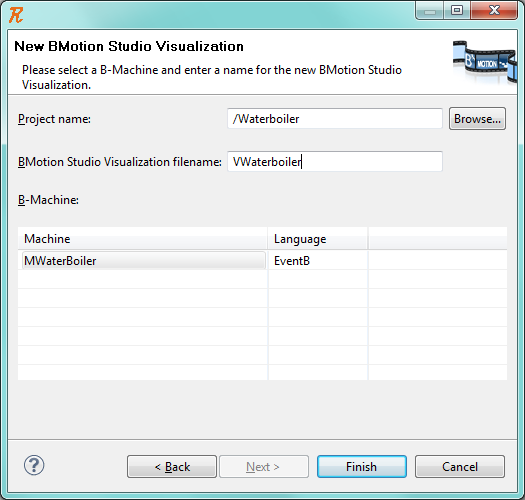
\includegraphics{img/tutorial/tut_03_waterboiler3.png}
	\caption{The New BMotion Studio Visualization wizard}
	\label{fig_tut_03_waterboiler3}
\end{center}
\end{figure}

Open the VWaterboiler file by double clicking on it. This should open the BMotion Studio editor. This part of the tutorial is finished. The next step in the tutorial is about working with Controls (\ref{tutorial_04}).
